\documentclass[a4paper,11pt]{article}
\usepackage[latin1]{inputenc}
\usepackage[T1]{fontenc}
\usepackage[english]{babel}
% \usepackage{amsmath}
% \usepackage{amssymb,amsfonts,textcomp}
% \usepackage{color}
% \usepackage{array}
% \usepackage{supertabular}
% \usepackage{hhline}
\usepackage{hyperref}
\usepackage{cite}
% \usepackage{etoolbox}
\usepackage{acro}
\usepackage{graphicx}
\usepackage[nodayofweek]{datetime}

\include{helpers/acronyms}
\DeclareGraphicsRule{*}{mps}{*}{}
\newcommand{\mparagraph}[1]{\paragraph{#1}\mbox{}\\}

% Commands
\newcommand{\HRule}{\rule{\linewidth}{0.5mm}} % Defines a new command for the horizontal lines

\begin{document}

	\begin{titlepage}
		\begin{centering}
		 
		%	HEADING SECTIONS
		\textbf{\textit{\large{B.Tech Project Report}}}\\[0.5cm]
		
		\textsc{\textbf{\LARGE{Decentralised Video Messenger
over a peer-2-peer Network }}}\\[1.5cm]

		\large{Submitted in partial fulfillment for the award of the Degree of Bachelor of Technology in Computer Science and Engineering}\\[1.5cm]

		\large{Submitted by}\\[0.5cm]

		\textbf{Raeesul Asad     (Roll No 13 400 046)}\\
		\textbf{Shamnas T. V.     (Roll No 13 400 054)}\\
                \textbf{Soorej Jones Pothoor     (Roll No 13 400 058)}\\
		\textbf{Jerry Raju     (Roll No 13 400 070)}\\[1.5cm]
		
		{Under the guidance of}\\[0.25cm]
		\large{Dr. Salim A.}\\[0.5cm]

		
\includegraphics[width=5cm]{images/logo.jpg} 

		Department of Computer Science and Engineering\\
		\textsc{College of Engineering, Trivandrum}\\
		\textsc{Kerala}\\
		\textsc{May 2017}\\
		\vfill % Fill the rest of the page with whitespace
		\end{centering}
	\end{titlepage}

	\begin{titlepage}
		\begin{centering}
			\textbf{\textit{\LARGE\textsc{{certificate}}}}\\
			
\includegraphics[width=4cm]{images/logo.jpg}\\
                        Department of Computer Science and Engineering\\
		\textsc{College of Engineering, Trivandrum}\\[1.0cm]

		\end{centering}

		\large{This is to certify that the project entitled ``Decentralised Video Messenger over a peer-2-peer Network'' is a bonafide record of the major project done by \textbf{Raeesul Asad} (Roll No. 13 400 046), \textbf{Shamnsas T. V.} (Roll No. 13 400 054)\textbf{Soorej Jones Pothoor} (Roll No 13 400 058) and \textbf{Jerry Raju} (Roll No 13 400 070) under my supervision and guidance, in partial fulfillment for the award of the Degree of Bachelor of Technology in Computer Science and Engineering from the University of Kerala for the year 2017.}\\[1.5cm]

		\begin{minipage}{0.4\textwidth}
		\begin{flushleft}
		\end{flushleft}
		\end{minipage}
		~
		\begin{minipage}{0.6\textwidth}
		\begin{centering} \large
		\large{Dr. Salim A.}\\
		\small{(Guide)}\\
		\small{\textit{\textbf{Associate Professor}}}\\
		\small{\textit{\textbf{Dept. of Computer Science and Engineering}}}\\[1.5cm]

		\large{Mrs. Liji P. I.}\\
		\small{\textit{\textbf{Professor and Head}}}\\
		\small{\textit{\textbf{Dept. of Computer Science and Engineering}}}\\
		\end{centering}
		\end{minipage}\\[1.0cm]

		\begin{flushleft}
		Place: Trivandrum\\
		Date:  11-05-2017\\
		\end{flushleft}
		\vfill % Fill the rest of the page with whitespace
	\end{titlepage}

	% TODO Ack before this
	\pagenumbering{roman}
	
	\begin{abstract}
In an age where communication is of paramount importance, it is considerably worrying that such networks are controlled by private companies. New information shows proof of an unprecedented amount of spying
on personal communications. It is in this context that we present the idea of a completely decentralised mode of video conferencing built over a peer-to-peer network, whose infrastructure is supported entirely by its users, and is secured using advanced cryptography. A purely peer to peer version of video communication would allow for communication to take place directly between the parties involved. Identities can be taken care of by using digital signatures. Distributed data structures hold the necessary information required to maintain the network and to form a communication channel between two nodes. Since the infrastructure is distributed over a p2p network, there is no cost associated with a dedicated server. The project uses concepts from multimedia encoding, peer-to-peer
networks, bittorrents(DHT protocol), VoIP, and distributed systems.\\

Peer to peer network model, a significant networking model after client-server model, has generated considerable academic interests due to its many properties. This project implements a fully functional peer to peer network built using TCP/IP, and provided excellent learning opportunities to study the subtleties and challenges of creating one such network.\\

The project as a stand alone application serves as a secure and decentralised communication tool, and may find application in fields where reliability, privacy and non interference are required.

	\end{abstract}
	
	\newpage
	\tableofcontents
	\newpage
	\listoffigures
	\newpage
	%\printacronyms[include-classes=abbrev,name=Abbreviations]
	\newpage

	\pagenumbering{arabic}
	\section{Introduction}
        \subsection{Motivation and Overview}
        In the light of recent news regarding government and corporate spying, and blatant disregard for personal data, a secure application for non-monitored and unlogged communication seemed to be an apparent necessity. With principles of freedom and privacy of the individual as primary objectives, the system was designed to ensure security, lack of central authority, reliability and privacy. A peer to peer network matched the requirements with its properties like decentralised architecture, and reliability. The system posed several challenges and subtleties during implementation which are of academic interest.\\

        The project is a decentralised video calling platform supported by a peer to peer network
much like a torrent network. Node machines run a software that connects the node to
the network. Pype uses asymmetric key cryptographic techniques to provide anonymity
and security. A decentralised network is resilient and harder to take down making it
more secure than a centralised client server based model. The system is also impartial as every node is identical and no node has more authority.

\subsection{Background and Literature Survey}
The project is an original creation inspired from several successful peer to peer applications such as BitTorrent, Bitcoin, and TOR Networks. Bittorrents are a peer to peer file sharing system. The DHT protocol used in BitTorrent inspired the AddrBook data structure used in this system. The Nakamoto consensus used in bitcoins for verifying authenticity of bitcoin blockchains is partially implemented to maintain consistency of dynamic data structures distributed over the network.\\

A significant obstacle to creating a peer to peer connection is the presence of NATs(Network Address Translators). NATs allow multiple applications and systems to operate using a single public IP address. A NAT allocates local IP addresses to devices connected to the NAT. Connections from these devices to the internet goes through, and its local IP address and port, along with its destination address and port is saved in a table with corresponding reassigned port. When a packet returns to device, the packet's source ip address, destination ip address and port are compared to that in the table and corresponding local ip address is reassigned to packet. When an IP packet from a source not on the table comes to a NAT, it is thrown away. It works well with the client-server network model, however causes issues with a peer to peer model since both peers could potentially be behind NATs. This issue is addressed using a scheme known as hole punching or NAT traversal. To open a NAT, a support server is used. When a peer requires a connection to an other peer, a request is sent to a server. The server is assumed to be connected to the other peer, and sends it a request. The recipient peer tries to establish a connection with the requesting peer. Since the requesting peer is already trying to establish connection, NAT is open for the requesting peer. When the other peer tries to establish a connection, its NAT is also opened and a connection is formed.

	\section{Design}
        \subsection{Operations}
        Once the application begins running, it tries to establish a connection with the support server to obtain its public IP address. It then requests a first peer to enter the network. Once connection is established to the first peer, it connects to more peers on the network. The user is presented with a window with options to Add Contact, generate new keys, select current keys, copy current keys and Make calls to user. If a call is made, it checks the address book entry corresponding to the callee hash address and decrypts the signature o discover callee node. A call request is sent to the callee node and awaits request accept. If request is accepted, the user is presented with a calling screen that contains video of user and video feed from the callee node, and an option to disconnect.
        \subsection{Data structures}
Implementation of Pype requires a few tailored data structures. They are
\begin{itemize}
\item Address Book (AddrBook)
%\item Call list
\item Peer list (peer\_list)
\end{itemize}
\subsubsection{Address Book}
Address book is a distributed document stored on each peer in the network. It is a map contains encrypted contact information indexed using  a hash of individual public keys used to uniquely identify a person. It is periodically updated. 
\begin{center}
  \begin{tabular}{ | c | c | }
    \hline
    hash\_addr & encrypted net\_addr\\
    \hline
  \end{tabular}
\end{center}
hash\_addr (Hash address)  is a 256 bit sha256 hash of a public key generated by the corresponding peer. Each peer has a pair of public key and private key.
cypherText is a plain-text encrypted using the private key corresponding to the public key used to make hash\_addr. The cypherText acts as a signature for the peer. The plain-text contains contact information and a meta data field as shown in the following format.
\begin{center}
  \begin{tabular}{ | c | }
    \hline
    meta\_data\\
    \hline
    net\_addr\\
    \hline
    hash\_addr\\
    \hline
  \end{tabular}
\end{center}
addr\_book[hash\_addr] returns corresponding cypherText or null if hash\_addr does not exist.
cypherText can be decrypted using the corresponding pub\_key.
The address book is maintained and synchronized by all peers. When a change occurs in the AddrBook of a node, the change is copied to a string called AddrBookDelta, and AddrBookDelta is published to all peers. On receiving an AddrBookDelta, the node checks its update history to see if the new Delta was previously received. If not, it is added to history and updates its AddrBook.
    
%\subsection{Call list}
%Call list is a list of tuples containing hash_addr of callee and caller.
%\begin{center}
%  \begin{tabular}{ | c | c | }
%    \hline
%    callee_hash_addr & caller_hash_addr\\
%    \hline
%  \end{tabular}
%\end{center}
%The call list is updated along with the address book and each peer checks to% see if its address is among the list of callees.
%The call list is maintained and synchronised by all peers.

\subsubsection{Peerlist}
Peerlist is a list of ip addresses to which a peer is connected to. The peerlist, found on each peer is the backbone of the Pype network. peerlist is independently maintained by each peer.
\begin{center}
  \begin{tabular}{ | c | c | }
    \hline
    peer1 net\_addr & control\_flags\\
    \hline
    peer2 net\_addr & control\_flags\\
    \hline
    ... & ...\\
    \hline
    peerN net\_addr & control\_flags\\
    \hline
  \end{tabular}
\end{center}



\subsection{Network}


\begin{figure}[H]
\begin{center}
  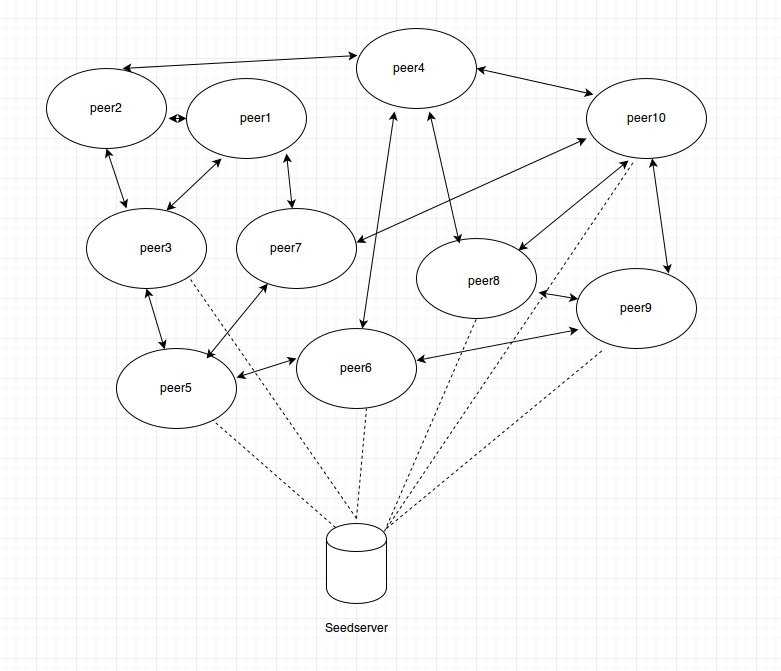
\includegraphics[width=0.60\textwidth]{images/network.png}
  \caption{2.3 - A sample network}
\end{center}
\end{figure}


Peer-to-peer (P2P) computing or networking is a distributed application architecture that partitions tasks or work loads between peers. Peers are equally privileged, equipotent participants in the application. They are said to form a peer-to-peer network of nodes.Peers make a portion of their resources, such as processing power, disk storage or network bandwidth, directly available to other network participants, without the need for central coordination by servers or stable hosts.Peers are both suppliers and consumers of resources, in contrast to the traditional client-server model in which the consumption and supply of resources is divided.

However, because of the widespread use of NAT architecture, our network cannot be truly decentralised. The network uses a seed server to bypass NAT restrictions and act as the entry point to the network.


\subsection{Interfaces}
\subsubsection{SupportServer}
The support server provides the following function calls
\begin{itemize}
\item \emph{net\_addr} getFirstPeer()
\item \emph{bool} getcon(string peer\_ip\_addr)
\item \emph{net\_addr} findMyIP()
\end{itemize}

\subsubsection{Peer}
The peer software provides the following function calls for accessing nodes.
\begin{itemize}
\item \emph{bool} newPeerRequest(string peer\_ip\_addr)
\item \emph{addr\_book} getAddressBook()
\item \emph{peer\_list} getPeerList()
\item \emph{bool} connect2call()
  \item \emph{bool} pushAddrBookDelta(AddrBookDelta)
\end{itemize}

\subsection{Architecture}

\subsubsection{Protocol Architecture}



The architecture includes a support server and a collection of peers. A peer runs a software that enables it to connect and communicate with the network. Since the NAT prevents nodes from forming direct connections, Pype uses a support server. A new peer connects to the support server and requests an entry node or a first peer. The support server provides a first peer. The node then asks the server to help make a connection to the first peer. The peer maintains a connection with the support server by occasionally polling and checking for connection requests, which allows the support server to communicate with the peer behind a NAT, since the address of the support server remains registered on the NAT. To connect to a node on the network, the peer requests a connection to the support server and sends packets to the node's ip address. These packets are ignored by the NAT on the router closest to the destination node. The support server sends a message to the node which contains the ip address of the requesting peer. This message gets through since its source ip address is already registered in the NAT of the destination node. The node tries to connect to the requesting peer by sending a message to its ip address. Since, the ip of the node is already in the NAT of the requesting peer, the message gets through. When the node sends a message to the source peer, the ip address of the source peer gets registered on the NAT of the destination node, enabling the source peer to communicate with the destination node and vice versa. The node requests a peer list from its first peer and connects to a few random nodes on the network. Once connected to a few nodes, the peer is a part of the Pype network. The peer also maintains a connection with the support server to enable new peers to connect to it.


After establishing its connections to the network, the peer asks for the address book. The address book is a data structure that holds a hash address and a cypherText field. The address book is updated throughout the network corresponding to changes occurring in any node in the network.




The address book contains two fields, and acts like a map. The first field is called the hash address. Each peer has a hash address. To create a hash address, the peer generates a pair of asymmetric keys. The sha256 hash of the public key is the hash address of the node. The cypherText field contains a plain-text that is encrypted using the peer's private key, and it contains it's ip address and some meta-data. Any changes to the AddrBook is broadcasted to the network as AddrBookDelta and every AddrBookDelta's hash is saved in a queue. When a new Delta is received, it is checked against the queue to see if the Delta was already added, in which case the Delta is discarded. Otherwise, the delta is added to current AddrBook and published again.


The network is anonymous because nobody can infer which ip contacts which other ip, unless they hold the public key of both peers. The network is also secure, because it uses encryption and defends itself from third party spying. Since the network is peer to peer that lacks a central server for supporting it, the network is resilient and protected from ddos and other attacks.

\subsubsection{Software Architecture}

\begin{figure}[H]
\begin{center}
  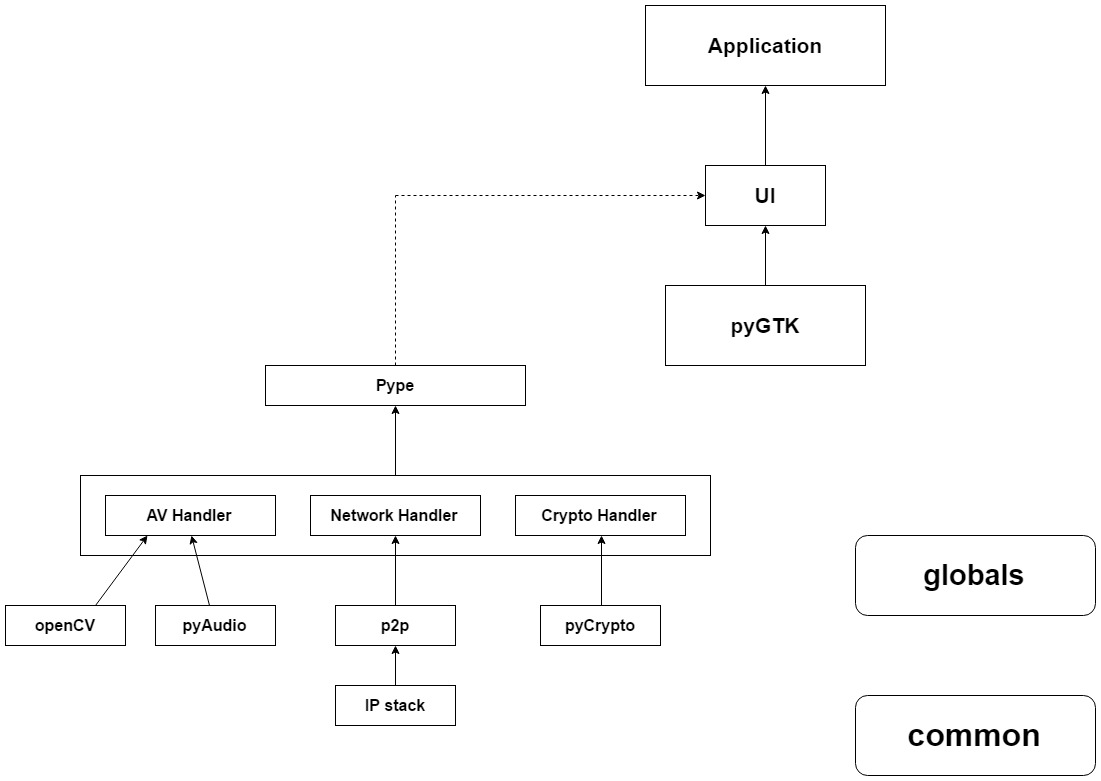
\includegraphics[width=0.60\textwidth]{images/pype.jpg}
  \caption{2.5.2 - Architecture}
\end{center}
\end{figure}

The software architecture is split into three major modules which form the application services layer.
\begin{itemize}
\item CryptoHandler\\ The CryptoHandler module is built using pycrypto library and acts as a wrapper for pycrypto. The CryptoHandler provides functionalities to generate signatures, decrypt signatures, create Hash Address,create SHA-256 hashes, encrypt text with AES, decrypt text with AES, base64 encoding, generate and manage RSA keys.
\item AVHandler\\ The AVHandler module was built using openCV and pyaudio. The module handles capturing video and audio from hardware, encoding the data stream, compressing it and sending it to the NetworkHandler. It also receives string streams from NetworkHandler, decodes audio and video and plays the result. The AVHandler module uses multiple threads to synchronize and manage Audio/Video.
Video and audio are received in one thread. It is the same thread
as sending video frame. This is to avoid thread starvation faced in
some computers. Used JPEG compression to reduce size of the video frame before
sending. (size approx:10kb) Audio is sent as such in chunks of 512 frames.
\item NetworkHandler\\The NetworkHandler module is built over a library called p2p, which in turn is implemented using TCP/IP. The p2p library handles NAT traversal, sending and receiving UDP packets to/from peers and support server. The NetworkHandler implements the Network protocol used in the project. It connects to different peers, maintains AddrBook, maintain network, and handle incoming connections. 

\end{itemize}

The common library contains definitions for custom data structures used in the project. The \_globals file contains all configuration variables and global variables. pyaudio, gtk, openCV, and pycrypto are external libraries used in building the project. p2p library was custom built to support NAT 
traversal. pyaudio is used to access audio devices. openCV is used to obtain video capture devices and display video. gtk is the application framework and window manager. pycrypto provides security services such as RSA, AES and DSS.


The pype module is built over the application services layer and handles most advanced protocol features. The pype module accesses CryptoHandler, AVHandler and NetworkHandler to make the application work. The UI object calls the pype object and creates the necessary UI.
It also runs the serverListenerThread which polls the server and receives information from the server, and the peerListenerThread which listens to peers. 



\section{Code Overview}
The code for the project is open on github: https://github.com/helioz/pype

\subsection{Programming Environment}
The application program is written entirely in python programming language. A desktop application framework called gtk is used to manage windows. The support server is written in C programming language and runs on a free VPS (Virtual Private Server). Python was chosen as default programming language because of the flexibility it provides. However, debugging and testing proved to be more challenging on python.

\subsection{Code Structure}
\begin{itemize}
\item Main.py
\item pype.sh
\item Documentation
  \begin{itemize}
  \item api
  \item Report
  \item SRS
  \end {itemize}
\item Resources
  \begin{itemize}
  \item \_globals.py
  \end{itemize}
  
\item lib
  \begin{itemize}
  \item common.py
  \item ui.py
  \item AVHandler.py
  \item CryptoHandler
  \item NetworkLib
    \begin{itemize}
    \item p2p.py
    \item NetworkHandler.py
    \item NetworkSupport.py
    \end{itemize}
  \end{itemize}  
\item tester
  \begin {itemize}
  \item Tests.py
  \item Diagnostics.text
  \item log.text
  \end{itemize}
\end {itemize}

\section{Results and Discussions}
\subsection{Result Observations}
The application runs successfully and all features implemented and described works. Due to the nature of p2p networks, starting the application has a significant delay due to the overhead of joining the network.

Since encoding was done using jpeg compression, each frame was compressed and sent. It is observable that a dynamic compression and encoding scheme such as x264 would yield better performance and smaller size for the AVstream.

Certain issues regarding compatibility of capturing audio was observed.

It is also observed that performance and reliability of the network is quite weak when number of nodes in the network is smaller than three. Due to the design, reliability, and security increases as number of nodes increases. 

\subsection{Screenshots}
\begin{figure}[H]
\begin{center}
  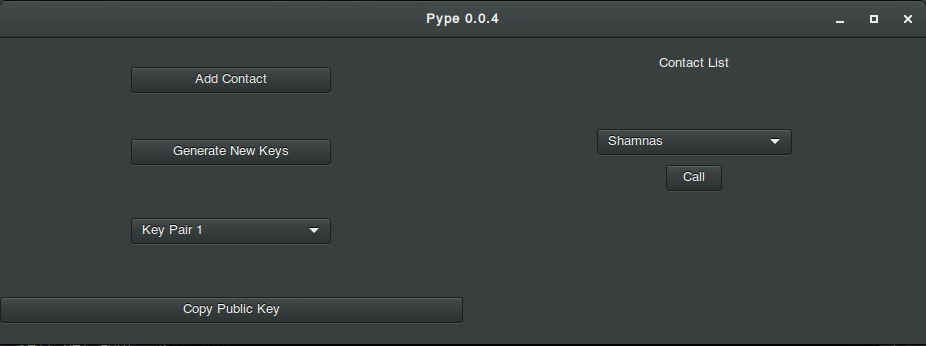
\includegraphics[width=1\textwidth]{images/homeScreen.png}
  \caption{Home screen}
\end{center}
\end{figure}
\begin{figure}[H]
\begin{center}
  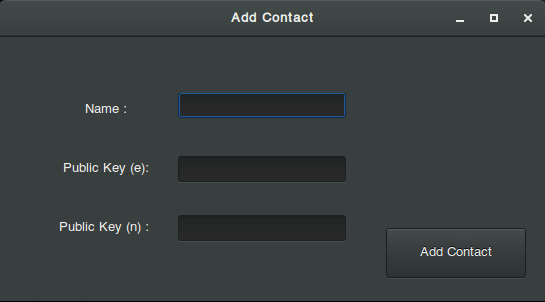
\includegraphics[width=0.50\textwidth]{images/addContactScreen.png}
  \caption{Add Contact Screen}
\end{center}
\end{figure}
\begin{figure}[H]
\begin{center}
  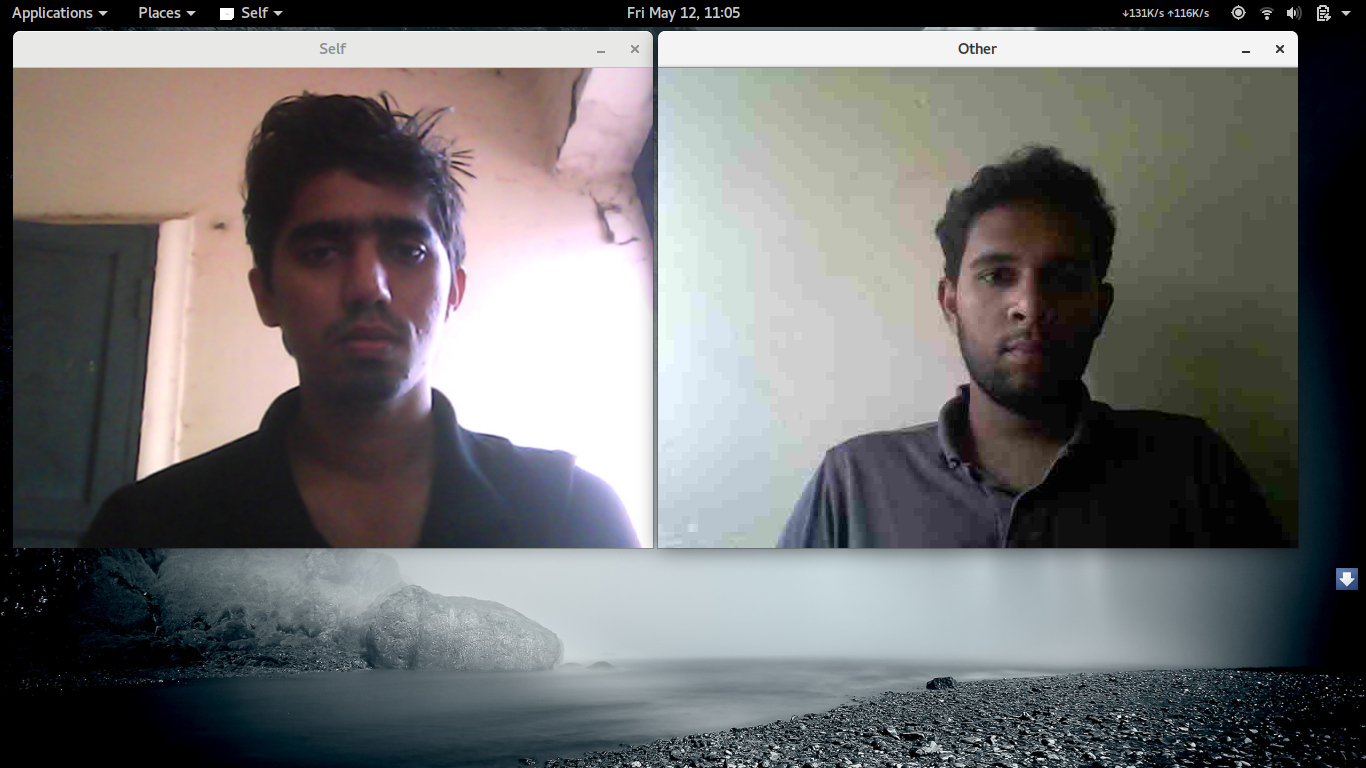
\includegraphics[width=0.50\textwidth]{images/callScreen.png}
  \caption{Calling Screen}
\end{center}
\end{figure}

\section{Further Work and Applications}
\subsection{Applications}
The project may find use in places where privacy and reliability are paramount concerns. Since a peer to peer network is resilient to attacks (Unless all nodes are taken down, which is considerably hard). The implementation of p2p may also be used for making other peer to peer networks. The project is also reliable over an unreliable or untrustworthy network. This is particularly useful for journalists and whistle-blowers who needs to avoid government oversight in places where free speech and free press are attacked.
\subsection{Further Works}
Further development may be done on the following fields:
\begin{itemize}
\item Change openCV to something lighter and more ubiquitous, such as gstreamer.
\item Improve compatibility of audio capture.
\item Use x264 or other streamable codecs for AV encoding.
\item Implement a setup to identify dead peers.
\item Port application to android and windows.
\item Clean code and improve performance.
\end{itemize}
  
\section{Conclusion}
We have seen the issues raised by privacy invasion and the need for a decentralised means of using the internet. Even though there are many means out there which aims at this goal of secure internet, we cannot say they meet all our requirements. Video messaging is one such field where decentralised means of operation is not readily available, but still increasing amount of population highly depend on as a means of communication through internet. Pype was introduced as a solution to this problem.   

 We try to implement Pype as an efficient and innovative system that allows both user anonymity and security. We achieved in creating a peer-to-peer network with minimal server dependency. Several issues including hole punching, traffic minimisation etc. were addressed and we were able to overcome them to an extent of initial implementation. There is still room for imrpovements.

We were able to send video and audio in a good quality and synchronization over our p2p internet with a few number of peers. We expect an increased performance with a larger, p2p network.

Security features such as data encryption, signature are implemented successfully with the help of standard libraries.

Pype as we said will be cost efficient, simple and an innovative step in the present communication scenario.

Peer to peer network model, a significant networking model after the client-server model, has generated considerable academic interests due to its many properties. This project implements a fully functional peer to peer network built using TCP/IP, and provided excellent learning opportunities to study the subtleties and challenges of creating one such network.\\

The project as a stand alone application serves as a secure and decentralised communication tool, and may find application in fields where reliability, privacy and non interference are required.

	\newpage
	\nocite{*}
	\bibliography{helpers/bibliography}
	\bibliographystyle{ieeetr}

\end{document}